\documentclass{article}

\usepackage{hyperref}
\usepackage{geometry}
\usepackage{changepage}
\usepackage{graphicx}
\usepackage[export]{adjustbox}
\usepackage{titlesec}
\usepackage{xcolor}
\hypersetup{
    colorlinks,
    linkcolor={red!50!black},
    citecolor={blue!50!black},
    urlcolor={blue!80!black}
}

\setlength\parindent{0pt} % noindet
\setcounter{secnumdepth}{4}

\geometry{legalpaper, margin=1in}

\graphicspath{{../img/}}

\titleformat{\paragraph}
{\normalfont\normalsize\bfseries}{\theparagraph}{1em}{}
\titlespacing*{\paragraph}
{0pt}{3.25ex plus 1ex minus .2ex}{1.5ex plus .2ex}

\begin{document}

\large{\textbf{Dr Thomas Huet}}\\
\normalsize
Chercheur et gestionnaire de base de données EAMENA\\
\small
$\cdot$Endangered Archaeology in the Middle East and North Africa\\
\normalsize
Université d'Oxford, École d'archéologie\\
\small
$\cdot$2 South Parks Road, Oxford OX1 3TG, Royaume-Uni
\normalsize
\\
\smash{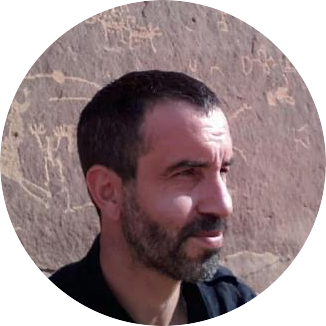
\includegraphics[width=3.5cm, right]{id-r}}

\includegraphics[scale=0.025]{gmail} \quad \href{mailto:thomas.huet@arch.ox.ac.uk}{thomas.huet@arch.ox.ac.uk} \& \href{mailto:thomashuet7@gmail.com}{thomashuet7@gmail.com}\\

\includegraphics[scale=0.01]{webpro} \quad \href{https://archit.web.ox.ac.uk/people/dr-thomas-huet}{École d'archéologie} \& \href{https://eamena.org/people/dr-thomas-huet}{Projet EAMENA}\\

\includegraphics[scale=0.007]{orcid} \quad \href{https://orcid.org/0000-0002-1112-6122}{0000-0002-1112-6122} \\

\includegraphics[scale=0.007]{github} \quad \href{https://github.com/zoometh/thomashuet.github.io/blob/main/README.md}{zoometh} \\

\includegraphics[scale=0.025]{gscholar} \quad \href{https://scholar.google.fr/citations?user=2hKEVaIAAAAJ}{2hKEVaIAAAAJ} \\

\includegraphics[scale=0.05]{rgate} \quad \href{https://www.researchgate.net/profile/Thomas\_Huet2}{Thomas\_Huet2} \\

\includegraphics[scale=0.005]{phone} \quad  \+ 44 (0)7 518 152 642 \\

\\

\begin{adjustwidth}{50pt}{50pt}
\begin{center}
\large{\textbf{Curriculum Vitae}}\\
\large{Préhistoire, patrimoine culturel et archéologie computationnelle} 
\end{center}
\end{adjustwidth}

\section{POSTES ACADEMIQUES ET PROFESSIONNELS (2014-)}

\textbf{depuis 2021 }Chercheur et gestionnaire de base de données EAMENA, Université d'Oxford, École d'archéologie, 2 South Parks Road, Oxford OX1 3TG, Royaume-Uni, 1er novembre-...
\smallbreak
\textbf{2021 }Technicien de soutien à la recherche spécialisé, Département de Préhistoire, Universitat Autònoma de Barcelona (UAB), Espagne, 1er juillet-31 décembre.
\smallbreak
\textbf{2020 }Co-responsable de l'étude des gravures médiévales de Sauri (Catalogne, Espagne), 2ème campagne, Universitat Autònoma de Barcelona (UAB), Espagne, 19 octobre-24 octobre.
\smallbreak
\textbf{2019-20 }Chercheur chez Archaïos, responsable de l'intégration de la base de données pour l'étude d'Al-'Ula, Arabie saoudite (Archaïos, AFALULA, RCU).
\smallbreak
\textbf{2019 }Co-responsable de l'étude des gravures médiévales de Sauri (Catalogne, Espagne), 1ère campagne, Universitat Autònoma de Barcelona (UAB), Espagne, 15 septembre-15 octobre.
\smallbreak
\textbf{--- }Concepteur de projet pour la création d'un pôle technologique en technologies émergentes pour les sciences humaines, UMR 8546 CNRS/PSL-AOrOc, Paris, resp. K. Gruel. 1er juin-1er juillet.
\smallbreak
\textbf{2018 }Ingénieur de recherche (IR), UMR 7264 CEPAM---CNRS, Université Nice Sophia-Antipolis, projet \textit{Céramiques Imprimées de Méditerranée occidentale} (CIMO), resp. D. Binder, 1er mai-30 août, et 1er octobre-30 novembre.
\smallbreak
\textbf{--- }Ingénieur de recherche (IR), UMR 5140, ASM-CNRS, Université Paul Valéry Montpellier 3, projet \textit{EpiSpat} (alias \textit{ArchaEpigraph}), LabEx ARCHIMEDE, resp. C. Pellecuer, 1er avril-1er mai, et 1er-30 septembre.
\smallbreak
\textbf{2017-8 }Formation sur les techniques d'enregistrement de l'art rupestre et des stèles gravées de la péninsule ibérique sud-ouest (\textit{Tecniques d'enregistrament de l'art rupestre de les esteles gravades del Sud-oest de la Peninsula ibèrica}), Grupo de investigación "Arqueología de las dinámicas sociales", Institución Milá y Fontanals (IMF) - Consejo Superior de Investigaciones Científicas (CSIC), Barcelone, resp. S. Valenzuela, 1er septembre 2017-30 mai 2018.
\smallbreak
\textbf{2017 }Développement du système d'information (SIG, base

 de données, topographie et photogrammétrie), grotte de Pertus II, Alpes-de-Haute-Provence, UMR 7264 CEPAM-CNRS, Université Nice Sophia-Antipolis et Evéha, resp. C. Lepère, 7-27 juillet.
\smallbreak
\textbf{2016 }Développement du système d'information (SIG, base de données, topographie et photogrammétrie), grotte de Pertus II, Alpes-de-Haute-Provence, UMR 7264 CEPAM-CNRS, Université Nice Sophia-Antipolis et Evéha, resp. C. Lepère, 1er-15 août 2016.
\smallbreak
\textbf{2015-6 }Chercheur postdoctoral, LabEx ARCHIMEDE, UMR 5140 ASM-CNRS et Université Paul-Valéry, Montpellier. Projet : "Étude des décors céramiques figuratifs de l'âge du bronze final dans le sud de la France et le nord-est de l'Espagne", 1er octobre 2015-30 septembre 2016.
\smallbreak
\textbf{2015 }Auditeur dans le séminaire de recherche "Regards croisés sur la notion de paysage", enseignant : S. Robert, EHESS, mars-juin.
\smallbreak
\textbf{2014 }Chargé de recherche (IR), projet \textit{Archaepigraph}, UMR 6249 Chrono-Environnement, Université de Franche-Comté, dir. M.-J. Ouriachi et L. Nuninger, 1er septembre-30 octobre.
\smallbreak
\textbf{2013-14 }Assistant de recherche (IE), USR CNRS -- UB 3516, plateforme GeoBFC, MSH de Dijon, Université de Bourgogne, projet OH-FET (Historical Object, Function, Space, Time), dir. L. Saligny, 1er juin-31 mai.

\section{FORMATION (2003-)}

\textbf{2006-12 }Doctorat en Histoire et Archéologie, titre : "Organisation spatiale et sériation des gravures piquetées du mont Bego", premier niveau de distinction (mention très honorable avec les félicitations du jury), 29 mai 2012, Université Nice Sophia-Antipolis, UMR 7264 CEPAM-CNRS, HALtheses: \href{https://tel.archives-ouvertes.fr/tel-00712290}{tel-00712290}.
\smallbreak
\textbf{2005-6 }Master 2 Recherche en Histoire et Archéologie, titre : "Étude des gravures protohistoriques de la zone des lacs (zones I, II, III et V) de la région du mont Bego, Tende, Alpes-Maritimes", mention bien, Université Nice Sophia-Antipolis, UMR 7264 CEPAM-CNRS, HALtheses: \href{https://tel.archives-ouvertes.fr/tel-00715386}{tel-00715386}.
\smallbreak
\textbf{2004-5 }DUT (Diplôme universitaire de technologie) en Génie Informatique, Conservatoire National des Arts et Métiers, Paris.
\small

break
\textbf{2003 }Diplôme de topographie, Universitad de Ingeniería, Lima, Pérou.

\section{PRIX ET DISTINCTIONS}

\textbf{2023 }Fonds Meyerstein.
\smallbreak
\textbf{2013 }Prix de thèse pour publication. CASDEN -- Banque Populaire (UFR LSH, Université Nice Sophia-Antipolis).

\end{document}